As Dennard scaling ends, big-data applications such as real-time image processing, graph analytics, and deep learning continue to push the boundaries of performance and energy efficiency requirements for compute system. 
One solution to this challenge is to move compute closer to memory or storage for substantial energy savings of data movement. 
We have developed an innovative Near-Data Computing (NDC) architecture that leverages the dramatic opportunities provided by the new CXL protocol. 
NDC incorporates heterogenous compute elements in the memory/storage subsystem to accelerate various computing tasks near data. 
One of these compute elements is the Streaming Engine (SE).

The SE is a Coarse-Grained Reconfigurable Array (CGRA) that is composed of interconnected compute tiles.  
The compute tiles are interconnected with both a Synchronous Fabric (SF) and an Asynchronous Fabric (AF) as shown in Fig. \ref{fig:se_diagram}.
It also interconnects tile memory, multiplexers, and Single Instruction Multiple Data (SIMD) units within each tile. 
Tiles can be pipelined through SF to form a synchronous data flow (SDF) through multiply/shift or add/logical SIMD units. 
AF connects a tile with all other tiles, dispatch interface (DI), and memory interfaces (MIs). 
It bridges SDFs through asynchronous operations, which include SDF initiation, asynchronous data transfer from one SDF to another, system memory accesses, and branching and looping constructs. 
Together, SF and AF allow the tiles to efficiently execute high-level programming language constructs. 
Simulation results of hand-crafted SE kernels have shown orders-of-magnitude better performance per watt on data-intensive applications than existing computing platforms.

Se example \ref{fig:se_example}
Mapping the instructions from the computation graph of a program onto the compute elements of the SE while adhering to architectural constraints is an NP-complete problem with a vast and sparse search space. 
Constraints related to tile memory and synchronous dataflow, use of delays to match timing requirements and more are necessary to ensure correct execution. 
Creating the mappings manually or using brute force algorithms takes time and lots of effort. 
This process also adds assumptions that reduce the search space, trading off optimization possibilities.  

In this work we propose a Deep Reinforcement Learning (RL) method to explore and find optimal mappings in an unsupervised manner. 
Using the Proximal Policy Optimization (PPO) method we train a neural network model to place instructions onto the SE tiles guided by a reward function that models the SE device and its constraints. 
The trained model was able to create valid mappings for the SE by learning about the problem domain. 
By using a learning methodology, we are able to reuse what the neural network learned to obtain mappings for computation graphs that were not seen during training.  

This work is motivated to provide improved tools set that lowers SE usability barrier. This also assist other tools or programmers in SE mapping creation by providing placement suggestions or tile 
configuration labels. The RL mapper performs unsupervised learning and optimization allowing it to search a wide and sparse search space. 

This line of research is inspired by recent work that used RL for chip placement. 
Our problem requirement of mapping nodes of a computation graph to available compute elements is similar to the problem of placing nodes of a chip netlist on a chip canvas. 

\begin{figure}
    \centering
    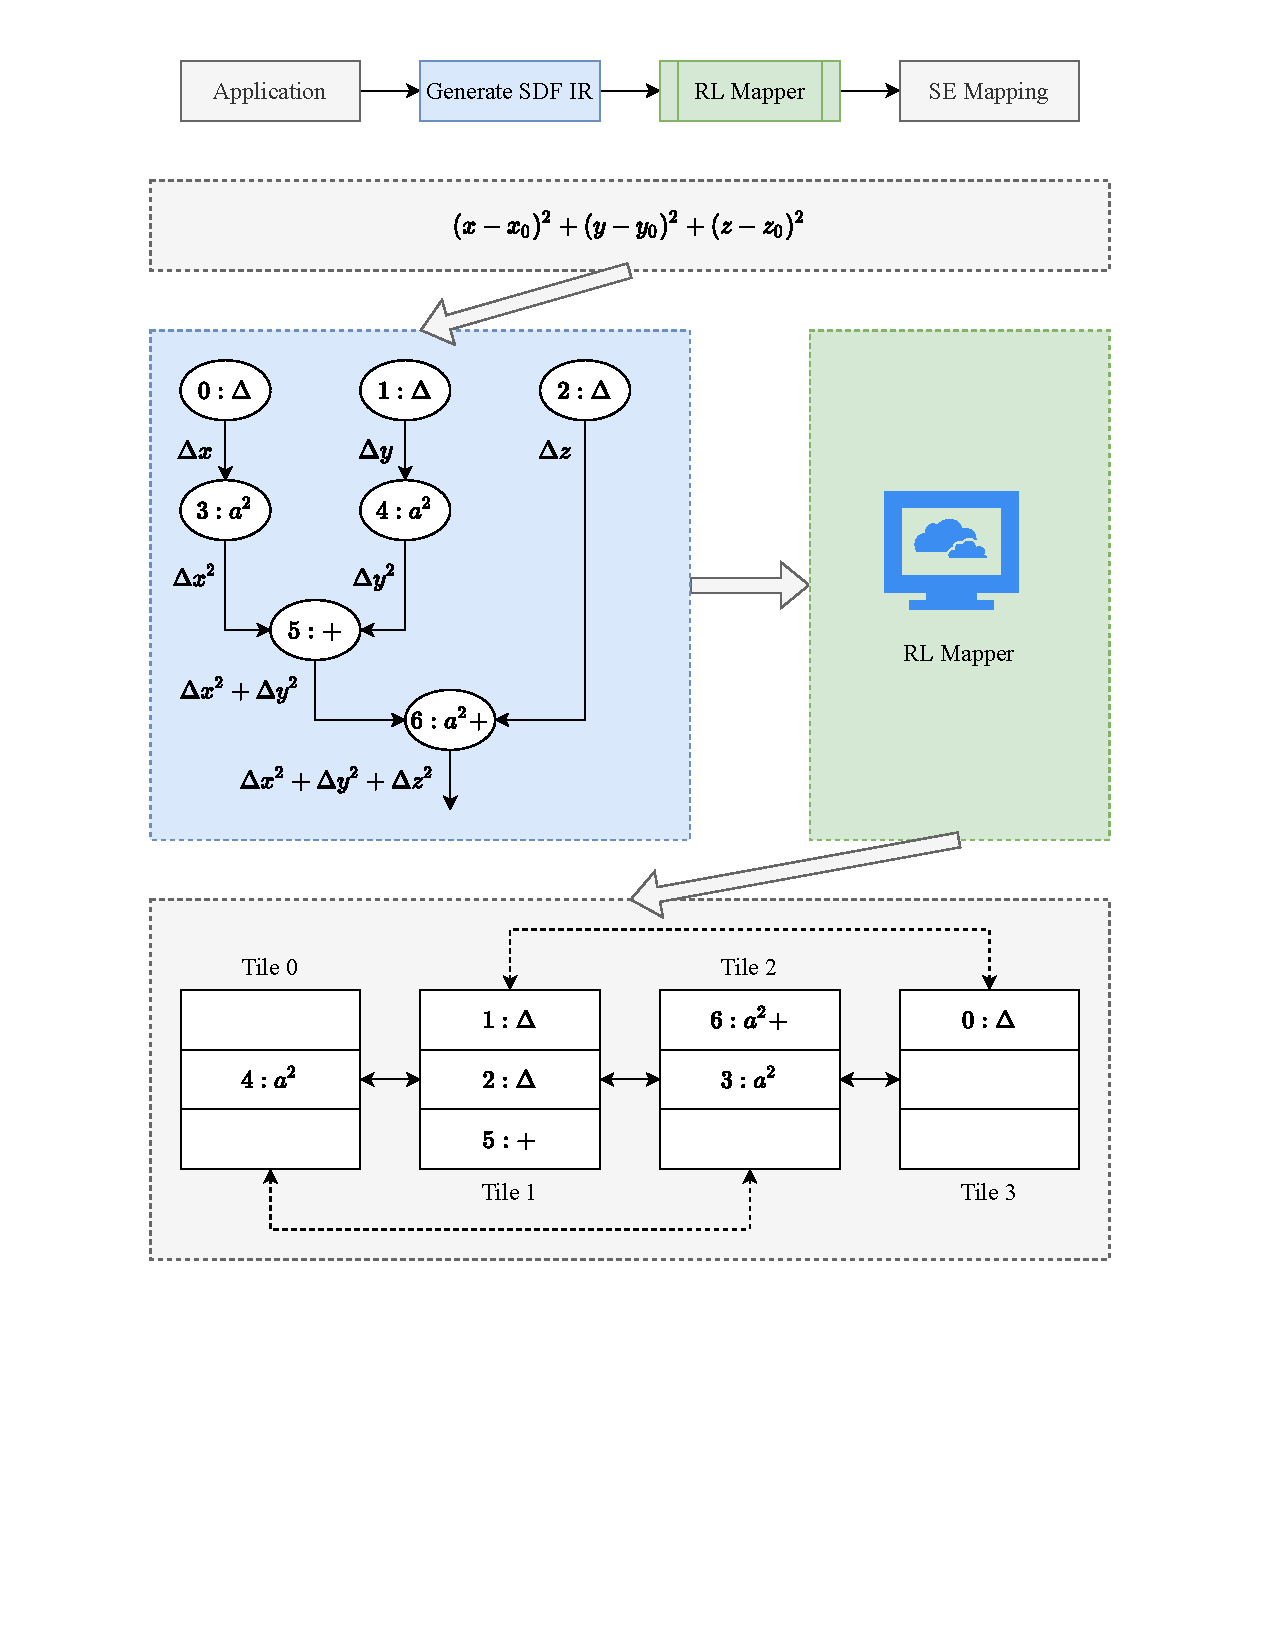
\includegraphics[width=\linewidth]{fig/SE_example.pdf}
    \caption{
      Diagram of the Streaming Engine.
    }
    \label{fig:se_example}
  \end{figure}